\documentclass[10pt,ignorenonframetext,]{beamer}
\setbeamertemplate{caption}[numbered]
\setbeamertemplate{caption label separator}{: }
\setbeamercolor{caption name}{fg=normal text.fg}
\beamertemplatenavigationsymbolsempty
\usepackage{lmodern}
\usepackage{amssymb,amsmath}
\usepackage{ifxetex,ifluatex}
\usepackage{fixltx2e} % provides \textsubscript
\ifnum 0\ifxetex 1\fi\ifluatex 1\fi=0 % if pdftex
  \usepackage[T1]{fontenc}
  \usepackage[utf8]{inputenc}
\else % if luatex or xelatex
  \ifxetex
    \usepackage{mathspec}
  \else
    \usepackage{fontspec}
  \fi
  \defaultfontfeatures{Ligatures=TeX,Scale=MatchLowercase}
\fi
\usetheme[]{Warsaw}
\usecolortheme{whale}
\usefonttheme{structuresmallcapsserif}
% use upquote if available, for straight quotes in verbatim environments
\IfFileExists{upquote.sty}{\usepackage{upquote}}{}
% use microtype if available
\IfFileExists{microtype.sty}{%
\usepackage{microtype}
\UseMicrotypeSet[protrusion]{basicmath} % disable protrusion for tt fonts
}{}
\newif\ifbibliography
\hypersetup{
            pdftitle={Einführung in R - Wie bekommt man Hilfe?},
            pdfauthor={Jan-Philipp Kolb},
            pdfborder={0 0 0},
            breaklinks=true}
\urlstyle{same}  % don't use monospace font for urls
\usepackage{color}
\usepackage{fancyvrb}
\newcommand{\VerbBar}{|}
\newcommand{\VERB}{\Verb[commandchars=\\\{\}]}
\DefineVerbatimEnvironment{Highlighting}{Verbatim}{commandchars=\\\{\}}
% Add ',fontsize=\small' for more characters per line
\usepackage{framed}
\definecolor{shadecolor}{RGB}{48,48,48}
\newenvironment{Shaded}{\begin{snugshade}}{\end{snugshade}}
\newcommand{\KeywordTok}[1]{\textcolor[rgb]{0.94,0.87,0.69}{#1}}
\newcommand{\DataTypeTok}[1]{\textcolor[rgb]{0.87,0.87,0.75}{#1}}
\newcommand{\DecValTok}[1]{\textcolor[rgb]{0.86,0.86,0.80}{#1}}
\newcommand{\BaseNTok}[1]{\textcolor[rgb]{0.86,0.64,0.64}{#1}}
\newcommand{\FloatTok}[1]{\textcolor[rgb]{0.75,0.75,0.82}{#1}}
\newcommand{\ConstantTok}[1]{\textcolor[rgb]{0.86,0.64,0.64}{\textbf{#1}}}
\newcommand{\CharTok}[1]{\textcolor[rgb]{0.86,0.64,0.64}{#1}}
\newcommand{\SpecialCharTok}[1]{\textcolor[rgb]{0.86,0.64,0.64}{#1}}
\newcommand{\StringTok}[1]{\textcolor[rgb]{0.80,0.58,0.58}{#1}}
\newcommand{\VerbatimStringTok}[1]{\textcolor[rgb]{0.80,0.58,0.58}{#1}}
\newcommand{\SpecialStringTok}[1]{\textcolor[rgb]{0.80,0.58,0.58}{#1}}
\newcommand{\ImportTok}[1]{\textcolor[rgb]{0.80,0.80,0.80}{#1}}
\newcommand{\CommentTok}[1]{\textcolor[rgb]{0.50,0.62,0.50}{#1}}
\newcommand{\DocumentationTok}[1]{\textcolor[rgb]{0.50,0.62,0.50}{#1}}
\newcommand{\AnnotationTok}[1]{\textcolor[rgb]{0.50,0.62,0.50}{\textbf{#1}}}
\newcommand{\CommentVarTok}[1]{\textcolor[rgb]{0.50,0.62,0.50}{\textbf{#1}}}
\newcommand{\OtherTok}[1]{\textcolor[rgb]{0.94,0.94,0.56}{#1}}
\newcommand{\FunctionTok}[1]{\textcolor[rgb]{0.94,0.94,0.56}{#1}}
\newcommand{\VariableTok}[1]{\textcolor[rgb]{0.80,0.80,0.80}{#1}}
\newcommand{\ControlFlowTok}[1]{\textcolor[rgb]{0.94,0.87,0.69}{#1}}
\newcommand{\OperatorTok}[1]{\textcolor[rgb]{0.94,0.94,0.82}{#1}}
\newcommand{\BuiltInTok}[1]{\textcolor[rgb]{0.80,0.80,0.80}{#1}}
\newcommand{\ExtensionTok}[1]{\textcolor[rgb]{0.80,0.80,0.80}{#1}}
\newcommand{\PreprocessorTok}[1]{\textcolor[rgb]{1.00,0.81,0.69}{\textbf{#1}}}
\newcommand{\AttributeTok}[1]{\textcolor[rgb]{0.80,0.80,0.80}{#1}}
\newcommand{\RegionMarkerTok}[1]{\textcolor[rgb]{0.80,0.80,0.80}{#1}}
\newcommand{\InformationTok}[1]{\textcolor[rgb]{0.50,0.62,0.50}{\textbf{#1}}}
\newcommand{\WarningTok}[1]{\textcolor[rgb]{0.50,0.62,0.50}{\textbf{#1}}}
\newcommand{\AlertTok}[1]{\textcolor[rgb]{1.00,0.81,0.69}{#1}}
\newcommand{\ErrorTok}[1]{\textcolor[rgb]{0.76,0.75,0.62}{#1}}
\newcommand{\NormalTok}[1]{\textcolor[rgb]{0.80,0.80,0.80}{#1}}
\usepackage{graphicx,grffile}
\makeatletter
\def\maxwidth{\ifdim\Gin@nat@width>\linewidth\linewidth\else\Gin@nat@width\fi}
\def\maxheight{\ifdim\Gin@nat@height>\textheight0.8\textheight\else\Gin@nat@height\fi}
\makeatother
% Scale images if necessary, so that they will not overflow the page
% margins by default, and it is still possible to overwrite the defaults
% using explicit options in \includegraphics[width, height, ...]{}
\setkeys{Gin}{width=\maxwidth,height=\maxheight,keepaspectratio}

% Prevent slide breaks in the middle of a paragraph:
\widowpenalties 1 10000
\raggedbottom

\AtBeginPart{
  \let\insertpartnumber\relax
  \let\partname\relax
  \frame{\partpage}
}
\AtBeginSection{
  \ifbibliography
  \else
    \let\insertsectionnumber\relax
    \let\sectionname\relax
    \frame{\sectionpage}
  \fi
}
\AtBeginSubsection{
  \let\insertsubsectionnumber\relax
  \let\subsectionname\relax
  \frame{\subsectionpage}
}

\setlength{\parindent}{0pt}
\setlength{\parskip}{6pt plus 2pt minus 1pt}
\setlength{\emergencystretch}{3em}  % prevent overfull lines
\providecommand{\tightlist}{%
  \setlength{\itemsep}{0pt}\setlength{\parskip}{0pt}}
\setcounter{secnumdepth}{0}

\title{Einführung in R - Wie bekommt man Hilfe?}
\author{Jan-Philipp Kolb}
\date{07 Juni, 2019}

\begin{document}
\frame{\titlepage}

\begin{frame}[fragile]{Wie bekomme ich Hilfe?}

\begin{itemize}
\tightlist
\item
  \href{http://itfeature.com/tag/how-to-get-help-in-r}{\textbf{Um Hilfe
  im Allgemeinen zu bekommen:}}
\end{itemize}

\begin{Shaded}
\begin{Highlighting}[]
\KeywordTok{help.start}\NormalTok{()}
\end{Highlighting}
\end{Shaded}

\begin{itemize}
\tightlist
\item
  \href{https://www.r-project.org/help.html}{\textbf{Online-Dokumentation
  für die meisten Funktionen:}}
\end{itemize}

\begin{Shaded}
\begin{Highlighting}[]
\KeywordTok{help}\NormalTok{(name)}
\end{Highlighting}
\end{Shaded}

\begin{itemize}
\tightlist
\item
  Benutze \texttt{?}, um Hilfe zu bekommen
\end{itemize}

\begin{Shaded}
\begin{Highlighting}[]
\NormalTok{?mean}
\end{Highlighting}
\end{Shaded}

\begin{itemize}
\tightlist
\item
  \texttt{example(lm)} liefert ein Beispiel für die lineare Regression
\end{itemize}

\begin{Shaded}
\begin{Highlighting}[]
\KeywordTok{example}\NormalTok{(lm)}
\end{Highlighting}
\end{Shaded}

\end{frame}

\begin{frame}[fragile]{Vignetten}

\begin{itemize}
\tightlist
\item
  Eine Vignette ist ein Papier, das die wichtigsten Funktionen eines
  Pakets darstellt.
\item
  Sie enthalten viele reproduzierbare Beispiele.
\item
  Vignetten sind ein neues Werkzeug, deshalb hat nicht jedes Paket eine
  Vignette.
\end{itemize}

\begin{Shaded}
\begin{Highlighting}[]
\KeywordTok{browseVignettes}\NormalTok{()}
\end{Highlighting}
\end{Shaded}

\begin{itemize}
\tightlist
\item
  Um eine Vignette zu bekommen:
\end{itemize}

\begin{Shaded}
\begin{Highlighting}[]
\KeywordTok{vignette}\NormalTok{(}\StringTok{"osmdata"}\NormalTok{)}
\end{Highlighting}
\end{Shaded}

\end{frame}

\begin{frame}{Ein Beispiel für eine Vignette - Das Paket
\texttt{osmdata}}

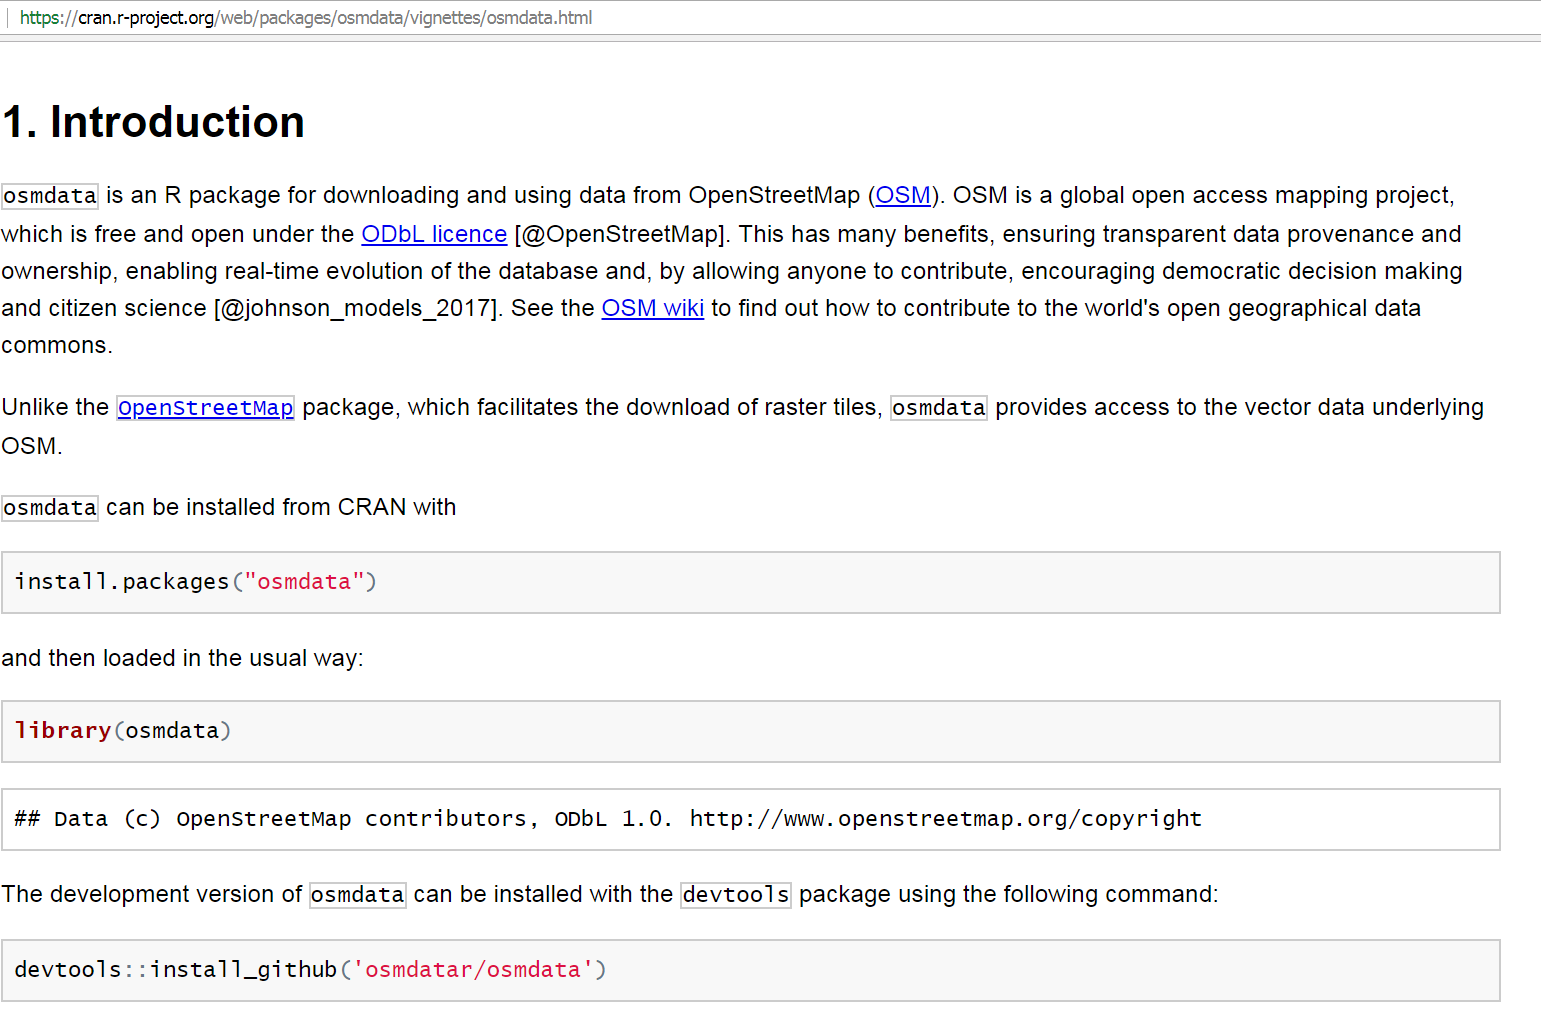
\includegraphics{figure/ex_osmdata_vignette.PNG}

\end{frame}

\begin{frame}[fragile]{\href{http://r-pkgs.had.co.nz/demo.html}{\textbf{Demos}}}

\begin{itemize}
\tightlist
\item
  für manche Pakete gibt es Demos:
\end{itemize}

\begin{Shaded}
\begin{Highlighting}[]
\KeywordTok{demo}\NormalTok{() }\CommentTok{# zeigt alle verfügbaren Demos}
\KeywordTok{demo}\NormalTok{(}\DataTypeTok{package =} \StringTok{"httr"}\NormalTok{) }\CommentTok{# Zeigt alle Demos in einem Paket}

\CommentTok{# Ein spezifisches Demo laufen lassen:}
\KeywordTok{demo}\NormalTok{(}\StringTok{"oauth1-twitter"}\NormalTok{, }\DataTypeTok{package =} \StringTok{"httr"}\NormalTok{) }
\end{Highlighting}
\end{Shaded}

\begin{itemize}
\tightlist
\item
  Wenn ein Demo gestartet wird, ist der zugehörige Code in der Konsole
  sichtbar
\end{itemize}

\begin{Shaded}
\begin{Highlighting}[]
\KeywordTok{demo}\NormalTok{(nlm)}
\end{Highlighting}
\end{Shaded}

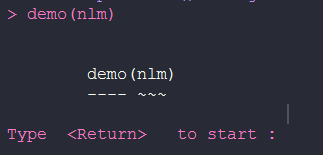
\includegraphics{figure/demonlm.PNG}

\end{frame}

\begin{frame}[fragile]{\href{http://www.r-tutor.com/r-introduction}{Die
Funktion \texttt{apropos}}}

\begin{itemize}
\tightlist
\item
  findet alles, was den angegebenen String enthält:
\end{itemize}

\begin{Shaded}
\begin{Highlighting}[]
\KeywordTok{apropos}\NormalTok{(}\StringTok{"nova"}\NormalTok{)}
\end{Highlighting}
\end{Shaded}

\begin{verbatim}
## [1] "anova"            "manova"           "power.anova.test"
## [4] "stat.anova"       "summary.manova"
\end{verbatim}

\begin{itemize}
\tightlist
\item
  Auch
  \href{https://de.wikipedia.org/wiki/Regul\%C3\%A4rer_Ausdruck}{\textbf{reguläre
  Ausdrücken}} können verwendet werden\ldots{}
\end{itemize}

\begin{Shaded}
\begin{Highlighting}[]
\NormalTok{?}\StringTok{"regular expression"}
\end{Highlighting}
\end{Shaded}

\begin{Shaded}
\begin{Highlighting}[]
\KeywordTok{help.search}\NormalTok{(}\StringTok{"^glm"}\NormalTok{)}
\end{Highlighting}
\end{Shaded}

\begin{itemize}
\tightlist
\item
  \texttt{??} ist ein Synonym für \texttt{help.search}
\end{itemize}

\end{frame}

\begin{frame}[fragile]{\href{http://search.r-project.org/cgi-bin/namazu.cgi?query=glm\&max=20\&result=normal\&sort=score\&idxname=functions\&idxname=vignettes\&idxname=views}{\textbf{Suchmaschine
für die R-Seite}}}

\begin{Shaded}
\begin{Highlighting}[]
\KeywordTok{RSiteSearch}\NormalTok{(}\StringTok{"glm"}\NormalTok{)}
\end{Highlighting}
\end{Shaded}

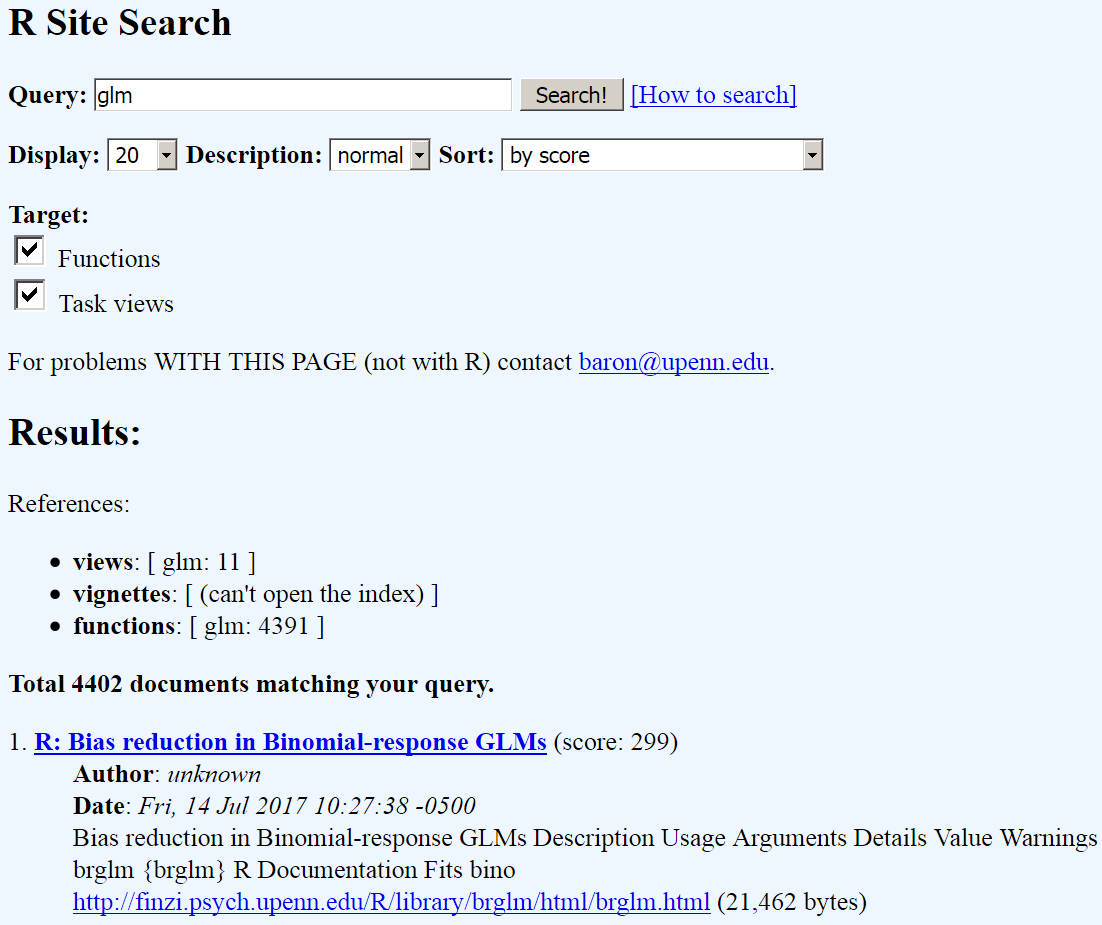
\includegraphics{figure/rsitesearch.PNG}

\end{frame}

\begin{frame}[fragile]{Nutzung von Suchmaschinen}

\begin{itemize}
\tightlist
\item
  Ich nutze \href{}{\textbf{duckduckgo.de:}}
\end{itemize}

\begin{verbatim}
R-project + "was ich schon immer wissen wollte" 
\end{verbatim}

\begin{itemize}
\tightlist
\item
  das funktioniert natürlich für alle Suchmaschinen!
\end{itemize}


\includegraphics{figure/duckduckgo.PNG}

\end{frame}

\begin{frame}{\href{http://stackoverflow.com/}{\textbf{Stackoverflow}}}

\begin{itemize}
\tightlist
\item
  Für alle Fragen zum Programmieren
\item
  Ist nicht auf R fokussiert - aber es gibt
  \href{https://stackoverflow.com/tags/r/info}{\textbf{viele
  Diskussionen zu R-Fragen}}
\item
  Sehr detailierte Diskussionen
\end{itemize}

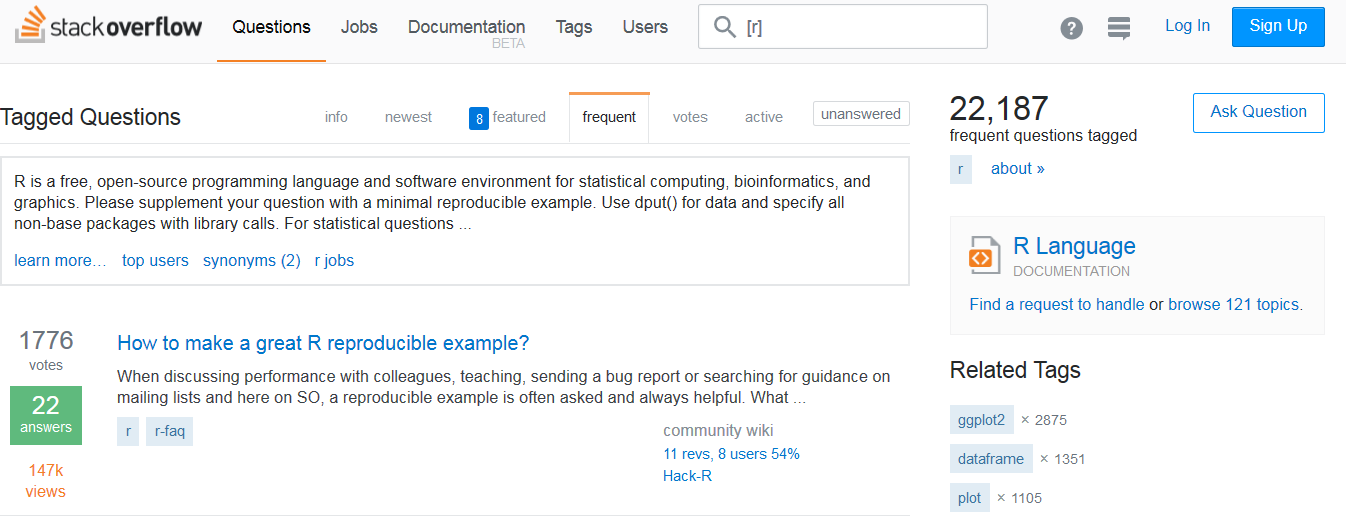
\includegraphics{figure/StackoverflowEx.PNG}

\end{frame}

\begin{frame}{Ein Schummelzettel für Basis R}

\url{https://www.rstudio.com/resources/cheatsheets/}

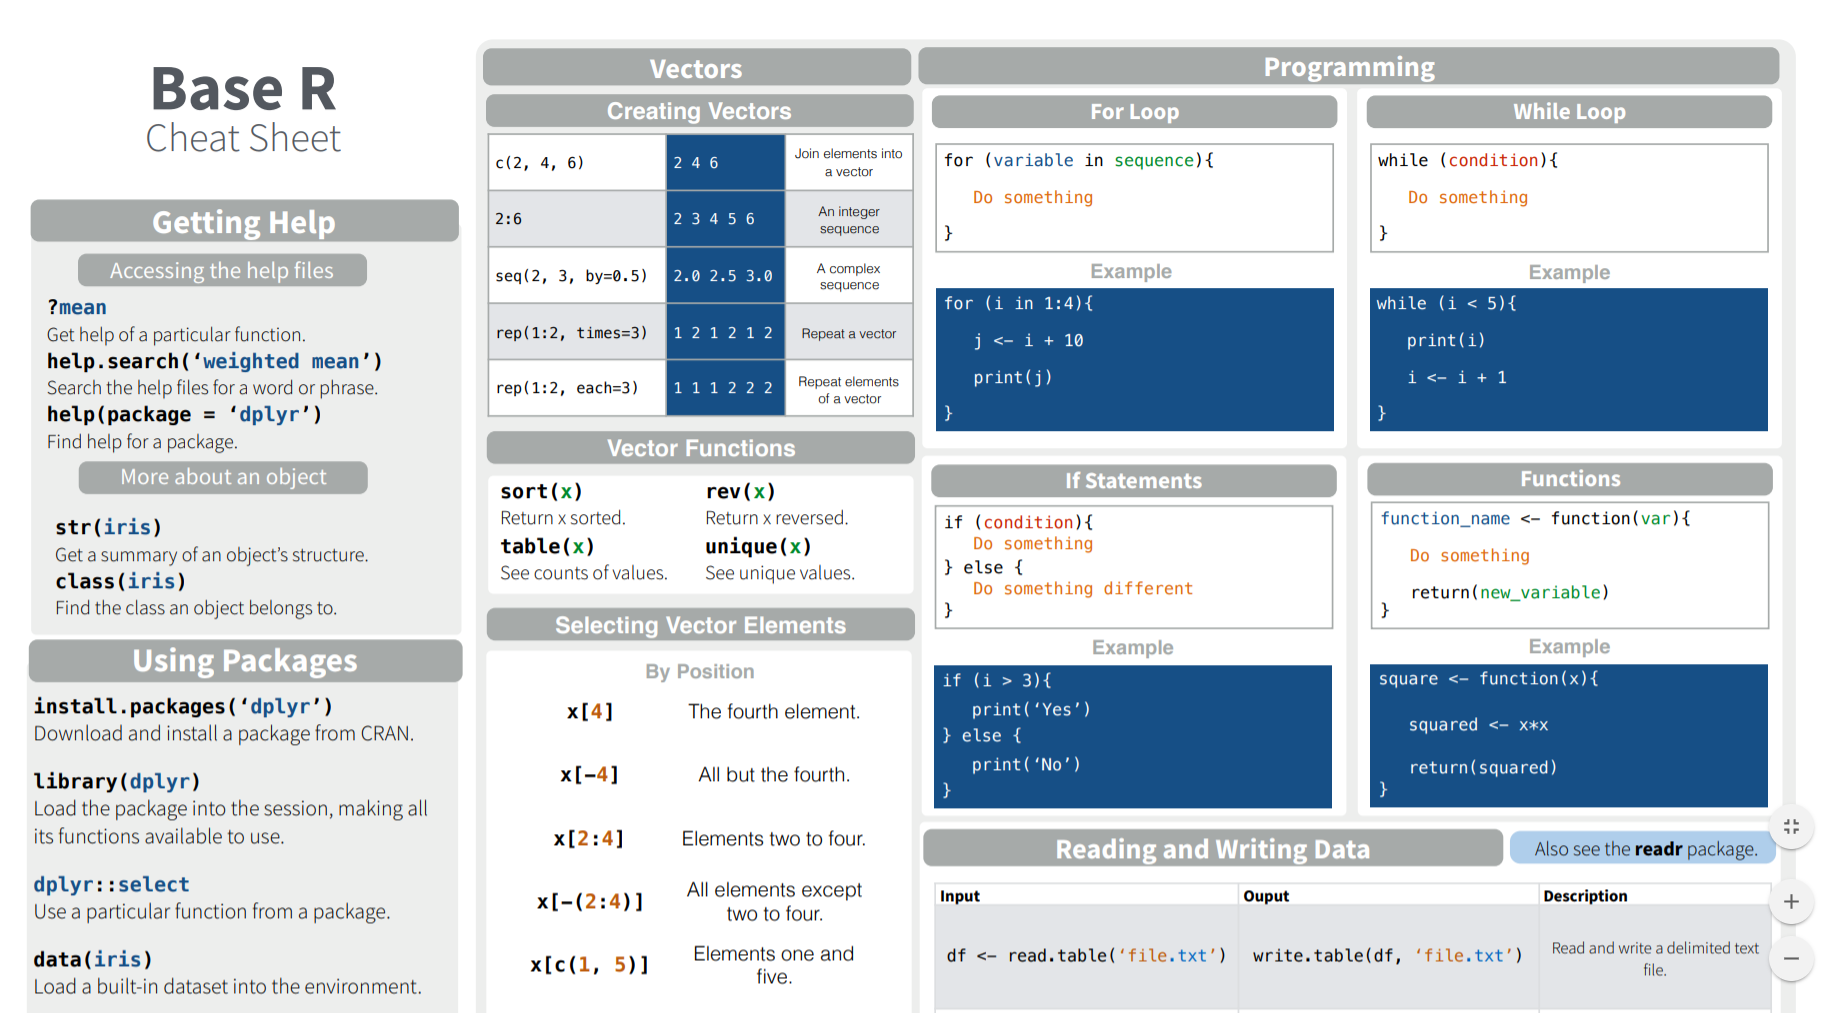
\includegraphics{figure/basercheatsheet.PNG}

\end{frame}

\begin{frame}{Mehr Schummelzettel}

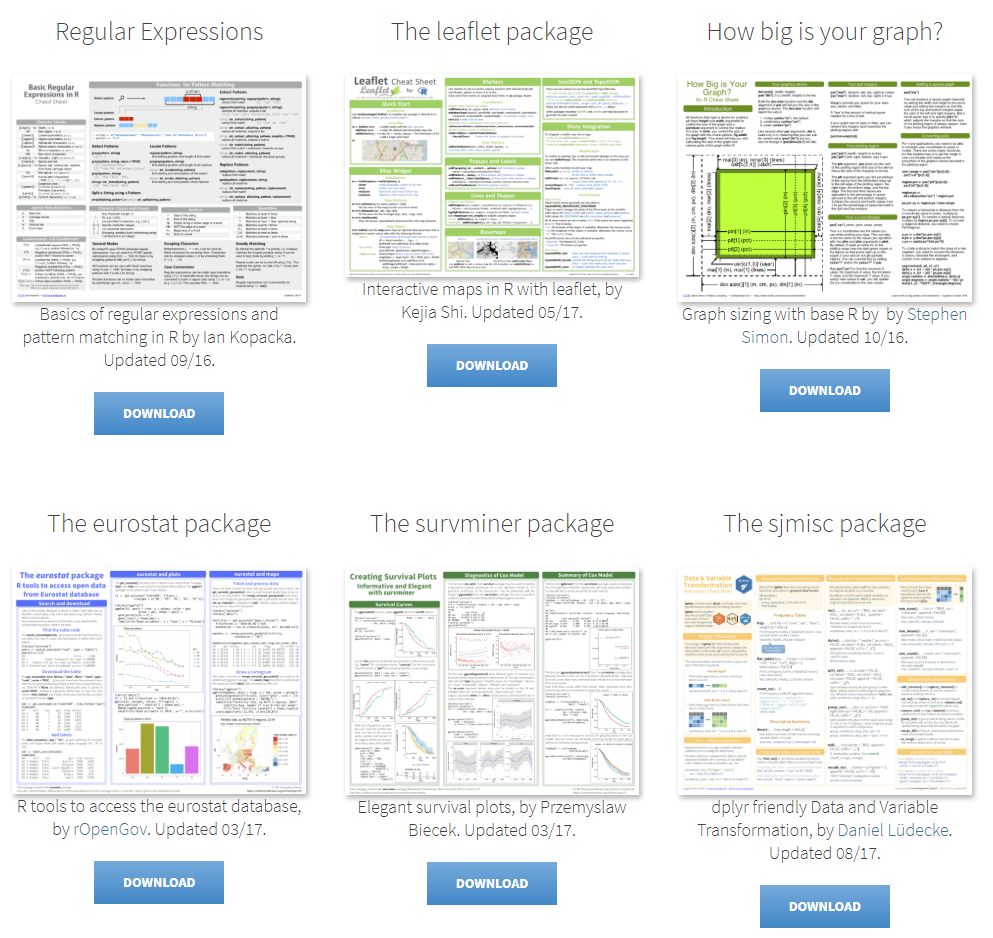
\includegraphics{figure/cheatsheets.PNG}

\end{frame}

\begin{frame}{\href{http://www.statmethods.net/interface/help.html}{\textbf{Quick
R}}}

\begin{itemize}
\tightlist
\item
  Viele Beispiele und Hilfe bezüglich eines Themas
\item
  Beispiel:
  \href{http://www.statmethods.net/interface/help.html}{\textbf{Quick R
  - Getting Help}}
\end{itemize}

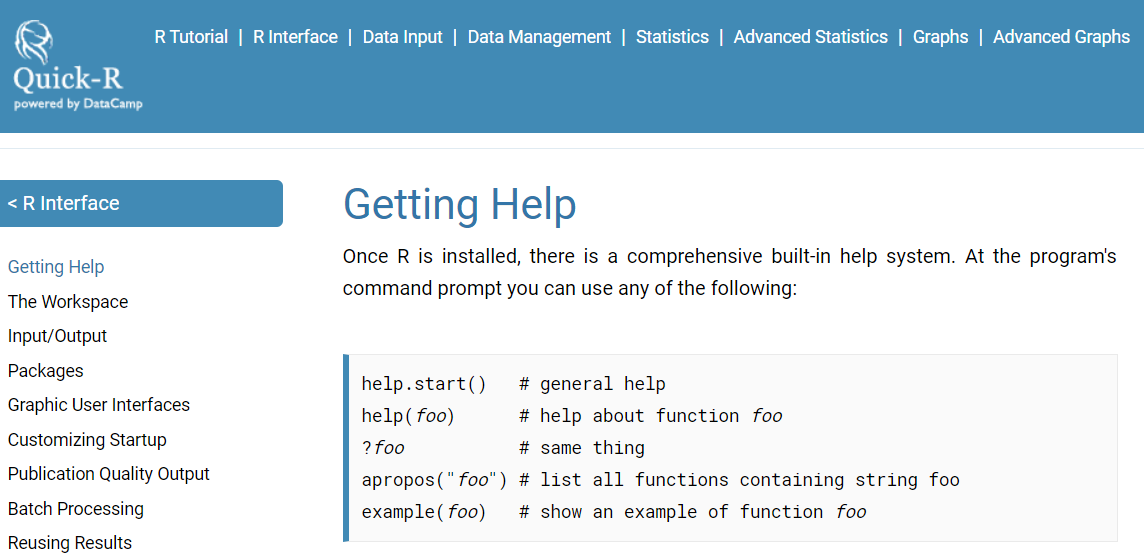
\includegraphics{figure/quickR.PNG}

\end{frame}

\begin{frame}{\href{https://swirlstats.com/}{Das Paket \texttt{swirl}}}


\includegraphics{figure/swirl.PNG}

\end{frame}

\begin{frame}[fragile]{Der Start mit \texttt{swirl}}

\begin{Shaded}
\begin{Highlighting}[]
\KeywordTok{library}\NormalTok{(swirl)}
\end{Highlighting}
\end{Shaded}

\begin{verbatim}
## Warning: package 'swirl' was built under R version 3.5.3
\end{verbatim}

\begin{verbatim}
## 
## | Hi! Type swirl() when you are ready to begin.
\end{verbatim}

\begin{Shaded}
\begin{Highlighting}[]
\KeywordTok{swirl}\NormalTok{()}
\end{Highlighting}
\end{Shaded}

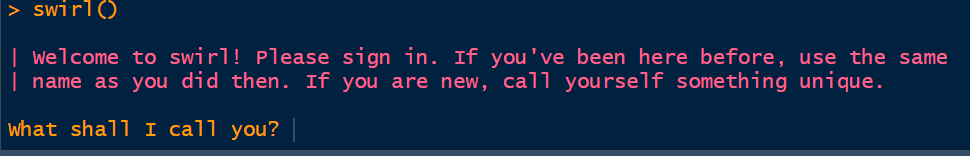
\includegraphics{figure/swirl_start.PNG}

\end{frame}

\begin{frame}{Weitere Links}

\begin{itemize}
\tightlist
\item
  \href{https://www.r-project.org/help.html}{\textbf{Überblick - wie
  bekommt man Hilfe in R}}
\end{itemize}


\includegraphics{figure/gettingHelp.PNG}

\begin{itemize}
\item
  \href{http://rprogramming.net/}{\textbf{Eine Liste mit HowTo`s}}
\item
  \href{https://www.personality-project.org/r/r.commands.html}{\textbf{Eine
  Liste mit den wichtigsten R-Befehlen}}
\end{itemize}

\end{frame}

\begin{frame}[fragile]{Aufgabe
\href{http://web.math.ku.dk/~helle/R-intro/exercises.pdf}{\textbf{Hilfe
bekommen}}}

\begin{block}{Hilfe für \texttt{which.min}}

\begin{itemize}
\item
  Tippe den Befehl \texttt{?which.min} in die Konsole. Dies öffnet eine
  Hilfeseite im unteren rechten Fenster von RStudio. Wofür kann man die
  Funktion \texttt{which.min} nutzen?
\item
  Der Name der Funktion muss bekannt sein, um die Hilfeseite so zu
  öffnen. Manchmal (oft, sogar) kennen man den Namen der R-Funktionen
  nicht; dann kann eine
  \href{https://duckduckgo.com/}{\textbf{Suchmaschine}} helfen. Suche
  bspw. mit den Begriffen \texttt{R\ minimum\ vector}.
\end{itemize}

\end{block}

\begin{block}{}

\begin{itemize}
\tightlist
\item
  Quelle: - LABORATORY FOR APPLIED STATISTICS: Intro to R -
  \href{http://web.math.ku.dk/~helle/R-intro/exercises.pdf}{\textbf{Exercises}}
\end{itemize}

\end{block}

\end{frame}

\end{document}
